\documentclass[12pt,a4paper]{report}
\usepackage{amsmath}
\usepackage{amssymb}
\usepackage{hyperref}
\usepackage{graphicx}
\usepackage{geometry}
\usepackage{tikz}
\usepackage{float}

\usetikzlibrary{external, shapes.geometric, arrows, arrows.meta}
\graphicspath{{images/}}

% \tikzexternalize[mode=list and make]

\tikzset{
    png export/.style={
        % First we call ImageMagick; change settings to requirements
        external/system call/.add={}{; magick convert -density 300 -transparent white "\image.pdf" "\image.png"},
        % Now we force the PNG figure to be used instead of the PDF
        /pgf/images/external info,
        /pgf/images/include external/.code={
            \includegraphics[width=\pgfexternalwidth,height=\pgfexternalheight]{##1.png}
        },
    }
}

% Define python style for highlighting code
\usepackage{listings}
\definecolor{deepgray}{rgb}{0.4, 0.4, 0.4}
\usepackage{color}
\definecolor{deepblue}{rgb}{0,0,0.5}
\definecolor{deepred}{rgb}{0.6,0,0}
\definecolor{deepgreen}{rgb}{0,0.5,0}

\definecolor{codegreen}{rgb}{0,0.6,0}
\definecolor{codegray}{rgb}{0.5,0.5,0.5}
\definecolor{codepurple}{rgb}{0.58,0,0.82}
\definecolor{backcolour}{rgb}{0.95,0.95,0.92}

\lstdefinestyle{graystyle}{
    backgroundcolor=\color{backcolour},   
    commentstyle=\color{codegreen},
    keywordstyle=\color{magenta},
    numberstyle=\tiny\color{codegray},
    stringstyle=\color{codepurple},
    basicstyle=\ttfamily,
    comment=[l]{\#},
    commentstyle=\color{deepgreen}\footnotesize\rmfamily,
    breakatwhitespace=false,         
    breaklines=true,                 
    captionpos=b,                    
    keepspaces=true,                 
    numbers=left,                    
    numbersep=5pt,                  
    showspaces=false,                
    showstringspaces=false,
    showtabs=false,                  
    tabsize=2
}

\lstdefinelanguage{Python}{
    keywords={and, as, assert, break, class, continue, def, del, elif, else, except, False, finally, for, from, global, if, import, in, is, lambda, None, nonlocal, not, or, pass, raise, return, True, try, while, with, yield},
    keywordstyle=\color{deepblue}\bfseries,
    ndkeywords={self},
    ndkeywordstyle=\color{deepgray}\bfseries,
    identifierstyle=\color{black},
    sensitive=true,
    comment=[l]{\#},
    commentstyle=\color{deepgreen}\ttfamily,
    stringstyle=\color{deepred}\ttfamily,
    morestring=[b]',
    morestring=[b]``
}
\lstdefinestyle{mystyle}{
    backgroundcolor=\color{white},
    commentstyle=\color{deepgreen},
    keywordstyle=\color{deepblue},
    numberstyle=\tiny\color{gray},
    stringstyle=\color{deepred},
    emphstyle=\ttb\color{deepred},
    basicstyle=\ttfamily,
    breakatwhitespace=false,
    breaklines=true,
    captionpos=b,
    keepspaces=true,
    numbers=left,
    numbersep=5pt,
    showspaces=false,
    showstringspaces=false,
    showtabs=false,
    tabsize=2
}
\lstset{style=mystyle}


\geometry{a4paper, margin=1in}

\title{Advantage of Quantum Computing in Breaking RSA Encryption}
\author{Your Name \\ Roll No: Your Roll Number \\ Guide: Guide Name}
\date{\today}

\begin{document}

\maketitle

\chapter*{Certificate}
This is to certify that the seminar report titled \textbf{Advantage of Quantum Computing in Breaking RSA Encryption} has been successfully completed by \textbf{Your Name}, Roll No: \textbf{Your Roll Number}, under the guidance of \textbf{Guide Name}. This report is submitted in partial fulfillment of the requirements for the seminar presentation.

\vspace{2cm}
\begin{flushright}
Signature of Guide \\
Signature of Student
\end{flushright}

\newpage

\tableofcontents
\newpage

\chapter*{Abstract}
Quantum computing has emerged as a revolutionary paradigm in computation, offering significant advantages over classical computing for certain types of problems. One of the most notable implications of quantum computing is its potential to break widely used cryptographic systems, such as RSA encryption. This report explores the principles of RSA encryption, the capabilities of quantum computing, and how quantum algorithms, particularly Shor's algorithm, pose a threat to the security of RSA\@. The report also discusses the implications of this threat and the need for quantum-resistant cryptographic systems.

\chapter{Introduction to RSA Encryption and Quantum Computing}

RSA encryption is a cornerstone of modern cryptography, widely used to secure digital communications. Its security is based on the computational difficulty of factoring large integers, a problem that classical computers find infeasible to solve within a reasonable timeframe. However, the advent of quantum computing introduces a paradigm shift in computational capabilities. Quantum computers, leveraging principles such as superposition and entanglement, can solve certain problems exponentially faster than classical computers. This chapter provides an overview of RSA encryption, its working principles, its critical role in ensuring secure communication, and the potential impact of quantum computing on its security.

\section{Overview of RSA Encryption}
RSA encryption, named after its inventors Rivest, Shamir, and Adleman, is a public-key cryptographic system that relies on two keys: a public key for encryption and a private key for decryption. The security of RSA is rooted in the mathematical challenge of factoring the product of two large prime numbers, which forms the basis of the private key.

\section{Working Principles of RSA}
The RSA algorithm involves three main steps:
\begin{enumerate}
    \item \textbf{Key Generation:} Two large prime numbers are chosen, and their product forms the modulus. The public and private keys are derived using modular arithmetic.
    \item \textbf{Encryption:} The sender uses the recipient's public key to encrypt the message, ensuring that only the recipient can decrypt it.
    \item \textbf{Decryption:} The recipient uses their private key to decrypt the message, recovering the original plaintext.
\end{enumerate}

\section{Role of RSA in Secure Communication}
RSA encryption is widely used in various applications, including:
\begin{itemize}
    \item Securing online transactions and communications.
    \item Authenticating digital signatures to verify the integrity of messages.
    \item Protecting sensitive data in email and file encryption.
\end{itemize}

\section{Introduction to Quantum Computing}
Quantum computing leverages the principles of quantum mechanics, such as superposition and entanglement, to perform computations. Unlike classical computers, which process information in binary bits, quantum computers use quantum bits (qubits) that can represent multiple states simultaneously.

\section{Impact of Quantum Computing on RSA}
The computational power of quantum computers poses a significant threat to RSA encryption. Quantum algorithms, such as Shor's algorithm, can factorize large integers exponentially faster than classical algorithms, rendering RSA insecure. This has profound implications for digital security and the need to develop quantum-resistant cryptographic systems.

This report will delve into the mathematical foundation of RSA encryption, the vulnerabilities of RSA to quantum attacks, and the implications of quantum computing on digital security. It will also explore the existing methods for breaking RSA encryption, the drawbacks of these methods, and the advantages of transitioning to quantum-resistant cryptographic systems. The report will conclude with a discussion on the future enhancements and applications of quantum-resistant cryptography.

\chapter{Background on RSA Encryption and Its Vulnerabilities}
The existing cryptographic systems, including RSA, rely on the computational difficulty of certain mathematical problems, such as integer factorization. Classical computers are unable to solve these problems efficiently, which forms the basis of RSA's security. This chapter discusses the existing system and its reliance on classical computational limitations.

\section{Mathematical Foundation of RSA}
The RSA cryptosystem, introduced by Rivest, Shamir, and Adleman in 1978~\cite{Rivest1978}, is based on the mathematical principles of number theory and modular arithmetic.

\section{Key Generation Process}
The RSA key generation process involves the following steps:
\begin{enumerate}
    \item Select two large prime numbers, \(p\) and \(q\).
    \item Compute their product, \(n = p \times q\), which serves as the modulus.
    \item Calculate the totient, \(\phi(n) = (p-1)(q-1)\).
    \item Choose a public exponent, \(e\), such that \(1 < e < \phi(n)\) and \(\gcd(e, \phi(n)) = 1\).
    \item Compute the private exponent, \(d\), as the modular multiplicative inverse of \(e\) modulo \(\phi(n)\), satisfying \(e \cdot d \equiv 1 \pmod{\phi(n)}\).
\end{enumerate}

As shown in Figure~\ref{fig:key_generation}, this process ensures the generation of secure keys for encryption and decryption.

\begin{figure}[ht!]
    \centering
    \tikzset{png export}
    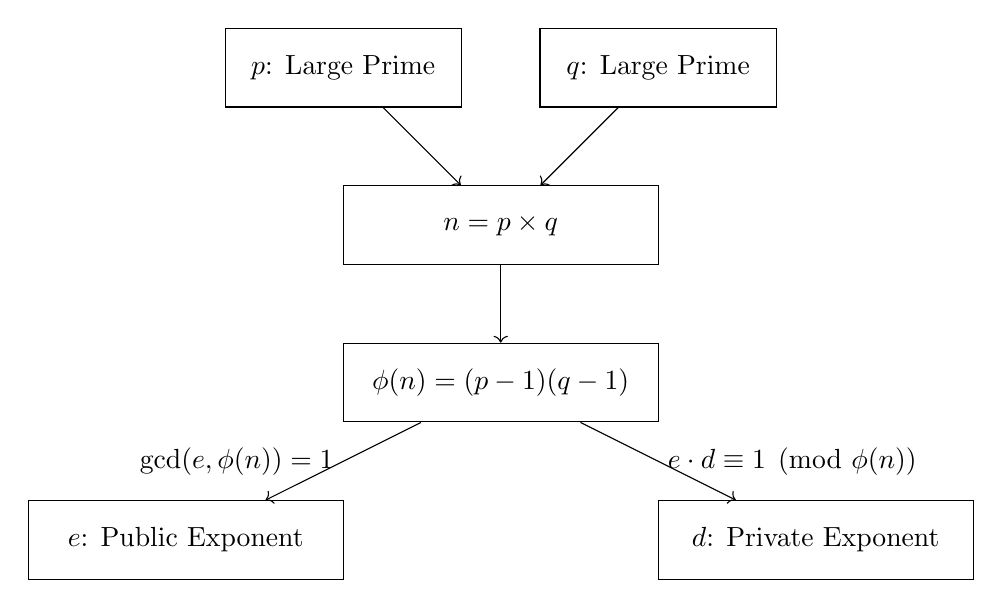
\begin{tikzpicture}
        % Draw the nodes
        \node[draw, rectangle, minimum width=3cm, minimum height=1cm] (p) at (0, 0) {\(p\): Large Prime};
        \node[draw, rectangle, minimum width=3cm, minimum height=1cm] (q) at (4, 0) {\(q\): Large Prime};
        \node[draw, rectangle, minimum width=4cm, minimum height=1cm] (n) at (2, -2) {\(n = p \times q\)};
        \node[draw, rectangle, minimum width=4cm, minimum height=1cm] (phi) at (2, -4) {\(\phi(n) = (p-1)(q-1)\)};
        \node[draw, rectangle, minimum width=4cm, minimum height=1cm] (e) at (-2, -6) {\(e\): Public Exponent};
        \node[draw, rectangle, minimum width=4cm, minimum height=1cm] (d) at (6, -6) {\(d\): Private Exponent};
        
        % Draw the arrows
        \draw[->] (p) -- (n);
        \draw[->] (q) -- (n);
        \draw[->] (n) -- (phi);
        \draw[->] (phi) -- (e) node[midway, left] {\(\gcd(e, \phi(n)) = 1\)};
        \draw[->] (phi) -- (d) node[midway, right] {\(e \cdot d \equiv 1 \pmod{\phi(n)}\)};
    \end{tikzpicture}
    \caption{Diagram illustrating the RSA key generation process.}%
    \label{fig:key_generation}
\end{figure}

\section{Encryption and Decryption Methods}
To encrypt a message \( M \) using a public encryption key \((e, n)\), proceed as follows:
\begin{enumerate}
    \item Represent the message as an integer between \( 0 \) and \( n-1 \). For long messages, break them into blocks and represent each block as such an integer.
    \item Encrypt the message by raising it to the \( e \)-th power modulo \( n \):
    \[
    C \equiv M^e \pmod{n},
    \]
    where \( C \) is the ciphertext.
\end{enumerate}

To decrypt the ciphertext \( C \), use the private decryption key \((d, n)\) and compute:
\[
M \equiv C^d \pmod{n}.
\]

Figure~\ref{fig:encryption_decryption} illustrates the encryption and decryption process.

\begin{figure}[h!]
    \centering
    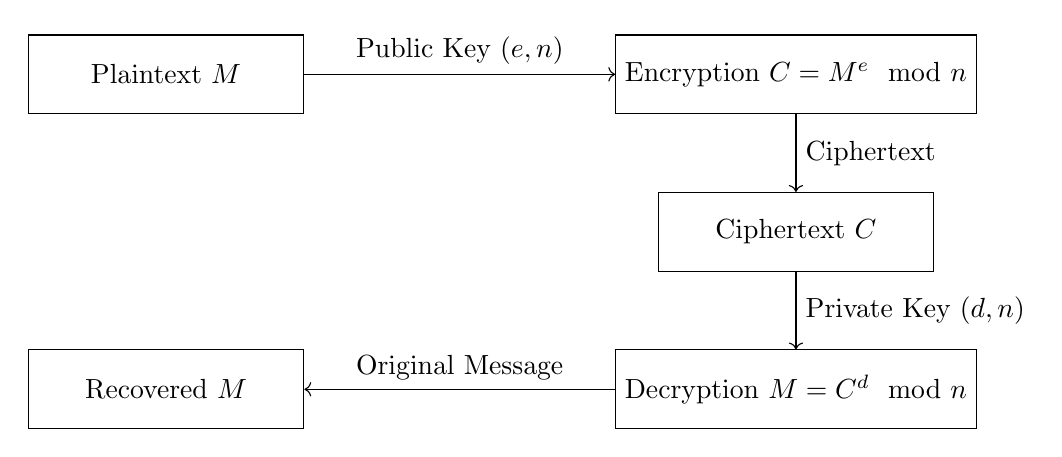
\begin{tikzpicture}
        % Nodes
        \node[draw, rectangle, minimum width=3.5cm, minimum height=1cm] (plaintext) at (0, 0) {Plaintext \(M\)};
        \node[draw, rectangle, minimum width=4.5cm, minimum height=1cm] (encryption) at (8, 0) {Encryption \(C = M^e \mod n\)};
        \node[draw, rectangle, minimum width=3.5cm, minimum height=1cm] (ciphertext) at (8, -2) {Ciphertext \(C\)};
        \node[draw, rectangle, minimum width=4.5cm, minimum height=1cm] (decryption) at (8, -4) {Decryption \(M = C^d \mod n\)};
        \node[draw, rectangle, minimum width=3.5cm, minimum height=1cm] (recovered) at (0, -4) {Recovered \(M\)};
        
        % Arrows
        \draw[->] (plaintext) -- (encryption) node[midway, above] {Public Key \((e, n)\)};
        \draw[->] (encryption) -- (ciphertext) node[midway, right] {Ciphertext};
        \draw[->] (ciphertext) -- (decryption) node[midway, right] {Private Key \((d, n)\)};
        \draw[->] (decryption) -- (recovered) node[midway, above] {Original Message};
        \end{tikzpicture}
    \caption{Diagram illustrating the RSA encryption and decryption process.}%
    \label{fig:encryption_decryption}
\end{figure}

\section{Example: Encrypting a Message Using RSA}
To illustrate the RSA encryption process, consider the following example:

\subsection{Key Generation}
\begin{itemize}
    \item Choose two prime numbers: \( p = 17 \) and \( q = 19 \).
    \item Compute \( n = p \times q = 17 \times 19 = 323 \).
    \item Calculate the totient: \( \phi(n) = (p-1)(q-1) = 16 \times 18 = 288 \).
    \item Select a public exponent \( e = 5 \), such that \( 1 < e < \phi(n) \) and \( \gcd(e, \phi(n)) = 1 \).
    \item Compute the private exponent \( d \), satisfying \( e \cdot d \equiv 1 \pmod{\phi(n)} \). Using the extended Euclidean algorithm, \( d = 173 \).
\end{itemize}

The public key is \( (e, n) = (5, 323) \), and the private key is \( (d, n) = (173, 323) \).

\subsection{Encryption of the Message}
To encrypt the message \texttt{Hello}, convert each character to its ASCII equivalent:
\begin{itemize}
    \item \texttt{H} = 72, \texttt{e} = 101, \texttt{l} = 108, \texttt{o} = 111.
\end{itemize}

Message is represented as: \texttt{[72, 101, 108, 108, 111]}.

\subsection{Encryption of the Message}
To encrypt the message \texttt{Hello}, convert each character to its ASCII equivalent:
\begin{itemize}
    \item \texttt{H} = 72, \texttt{e} = 101, \texttt{l} = 108, \texttt{o} = 111.
\end{itemize}

Encrypt each character \( M \) using the formula:
\[
C \equiv M^e \pmod{n}.
\]

\begin{itemize}
    \item For \texttt{H}: \( C \equiv 72^5 \pmod{323} = 21 \).
    \item For \texttt{e}: \( C \equiv 101^5 \pmod{323} = 271 \).
    \item For \texttt{l}: \( C \equiv 108^5 \pmod{323} = 109 \).
    \item For \texttt{o}: \( C \equiv 111^5 \pmod{323} = 42 \).
\end{itemize}

The encrypted message is represented as:
\[
\text{Ciphertext: } \texttt{[21, 271, 109, 109, 42]}.
\]

The corresponding encrypted text is:
\[
\text{Encrypted Message: } \texttt{§ďmm*}.
\]

\subsection{Decryption of the Message}
To decrypt the ciphertext, use the private key \( (d, n) = (173, 323) \) and the formula:
\[
M \equiv C^d \pmod{n}.
\]

\begin{itemize}
    \item For \( C = 21 \): \( M \equiv 21^{173} \pmod{323} = 72 \) (\texttt{H}).
    \item For \( C = 271 \): \( M \equiv 271^{173} \pmod{323} = 101 \) (\texttt{e}).
    \item For \( C = 109 \): \( M \equiv 109^{173} \pmod{323} = 108 \) (\texttt{l}).
    \item For \( C = 42 \): \( M \equiv 42^{173} \pmod{323} = 111 \) (\texttt{o}).
\end{itemize}

The decrypted message is \texttt{Hello}, demonstrating the correctness of the RSA encryption and decryption process.

\section{Mathematical Proof of Correctness}
The correctness of the decryption process is guaranteed by Euler's theorem, which states:
\[
M^{\phi(n)} \equiv 1 \pmod{n},
\]
for any integer \( M \) coprime to \( n \). Since \( e \cdot d \equiv 1 \pmod{\phi(n)} \), it follows that:
\[
M^{e \cdot d} \equiv M \pmod{n}.
\]
This ensures that decryption correctly recovers the original message \( M \).

\section{Very Large Primes in RSA}
The security of RSA encryption heavily relies on the use of very large prime numbers. These primes are chosen to ensure that the modulus \( n = p \times q \) is sufficiently large, making factorization computationally infeasible for classical computers.

\subsection{Properties of Large Primes}
Very large primes used in RSA have the following properties:
\begin{itemize}
    \item \textbf{Size:} Typically, primes are hundreds of digits long (e.g., 1024-bit, 2048-bit, or even larger primes in modern implementations). For example, a 200-digit \( n \) provides a strong margin of safety against classical attacks, while shorter lengths like 80 digits offer only moderate security.
    \item \textbf{Randomness:} Primes are generated randomly to avoid predictability, ensuring that attackers cannot guess or precompute potential primes.
    \item \textbf{Certainty:} Probabilistic primality tests, such as the Miller-Rabin test or the Baillie-PSW primality test, are used to ensure the numbers are prime with high confidence. Deterministic tests like the AKS primality test may also be used for absolute certainty, though they are computationally more expensive.
\end{itemize}

\subsection{Generation of Large Primes}
The process of generating large primes involves the following steps:
\begin{enumerate}
    \item \textbf{Random Selection:} Randomly select a large odd number within the desired range (e.g., 1024-bit or 2048-bit range).
    \item \textbf{Primality Testing:} Test the number for primality using efficient algorithms:
    \begin{itemize}
        \item \textbf{Miller-Rabin Test:} A probabilistic test that can quickly identify composite numbers. Multiple iterations increase the confidence level.
        \item \textbf{Lucas-Lehmer Test:} Often used for specific types of primes, such as Mersenne primes.
        \item \textbf{AKS Primality Test:} A deterministic test that guarantees correctness but is slower than probabilistic methods.
    \end{itemize}
    \item \textbf{Iteration:} If the number fails the primality test, repeat the process with a new candidate until a prime is found.
\end{enumerate}

\subsection{Challenges with Large Primes}
While the use of very large primes is essential for RSA security, it introduces several challenges:
\begin{itemize}
    \item \textbf{Computational Cost:} Generating and verifying large primes is computationally expensive, especially for key sizes of 4096 bits or more.
    \item \textbf{Storage and Transmission:} Large primes require more storage space and bandwidth for secure transmission, increasing the overhead in cryptographic systems.
    \item \textbf{Quantum Threats:} Despite the use of very large primes, RSA remains vulnerable to quantum algorithms like Shor's algorithm, which can efficiently factorize the modulus \( n \) and compromise the encryption.
\end{itemize}

\subsection{Importance of Large Primes in RSA}
The use of very large primes is a cornerstone of RSA encryption, ensuring its robustness against classical attacks. The difficulty of factoring the product of two large primes underpins the security of RSA, making it a reliable cryptographic standard for decades. However, the emergence of quantum computing necessitates the development of quantum-resistant alternatives to address the vulnerabilities posed by quantum algorithms.

% Python code for RSA encryption and decryption
\section{Python Implementation of RSA Encryption and Decryption}
The following Python code demonstrates the RSA encryption and decryption process:


As shown in Listing~\ref{lst:rsa_example_generic}, the Python implementation demonstrates the RSA encryption and decryption process.

\begin{lstlisting}[language=Python, caption=RSA Encryption and Decryption Example, label={lst:rsa_example_generic}]
# Function to compute modular exponentiation
def mod_exp(base, exp, mod):
    result = 1
    while exp > 0:
        if exp % 2 == 1:  # If exponent is odd
            result = (result * base) % mod
        base = (base * base) % mod
        exp //= 2
    return result

# RSA Key Generation
def generate_keys():
    p = 61  # Example prime number
    q = 53  # Example prime number
    n = p * q
    phi = (p - 1) * (q - 1)
    e = 17  # Public exponent (must be coprime with phi)
    d = pow(e, -1, phi)  # Private exponent (modular inverse of e mod phi)
    return (e, n), (d, n)

# RSA Encryption
def encrypt(message, public_key):
    e, n = public_key
    return [mod_exp(ord(char), e, n) for char in message]

# RSA Decryption
def decrypt(ciphertext, private_key):
    d, n = private_key
    return ''.join([chr(mod_exp(char, d, n)) for char in ciphertext])

# Example Usage
public_key, private_key = generate_keys()
message = "HELLO"
ciphertext = encrypt(message, public_key)
decrypted_message = decrypt(ciphertext, private_key)

print("Original Message:", message)
print("Encrypted Message:", ciphertext)
print("Decrypted Message:", decrypted_message)
\end{lstlisting}

As shown in Listing~\ref{lst:rsa_example}, the Python implementation demonstrates the RSA encryption and decryption process.

\begin{lstlisting}[language=Python, caption=Python code for RSA encryption and decryption, label={lst:rsa_example}]
from Crypto.Util.number import bytes_to_long, long_to_bytes
from Crypto.PublicKey import RSA
from Crypto.Random import get_random_bytes
from Crypto.Cipher import PKCS1_OAEP

# Generate RSA keys
key = RSA.generate(2048)
private_key = key.export_key()
public_key = key.publickey().export_key()

# Encrypt a message
message = b"Hello, Quantum World!"
cipher = PKCS1_OAEP.new(RSA.import_key(public_key))
ciphertext = cipher.encrypt(message)

# Decrypt the message
decipher = PKCS1_OAEP.new(RSA.import_key(private_key))
decrypted_message = decipher.decrypt(ciphertext)

# Print results
print("Original Message:", message)
print("Encrypted Message:", ciphertext)
print("Decrypted Message:", decrypted_message)
\end{lstlisting}

\section{Vulnerabilities of RSA}
While RSA is secure against classical attacks with sufficiently large key sizes, it has inherent vulnerabilities:
\begin{itemize}
    \item \textbf{Small Key Sizes:} RSA keys smaller than 2048 bits are susceptible to factorization using advanced classical algorithms.
    \item \textbf{Implementation Flaws:} Poor implementation practices, such as weak random number generation, can compromise RSA security.
    \item \textbf{Side-Channel Attacks:} Physical attacks exploiting timing, power, or electromagnetic emissions can reveal private keys.
    \item \textbf{Quantum Threats:} The advent of quantum computing introduces algorithms, such as Shor's algorithm, that can efficiently factorize large integers, rendering RSA insecure.
\end{itemize}

\section{Mitigation Strategies}
To address these vulnerabilities, several strategies have been proposed, as depicted in Figure~\ref{fig:mitigation_strategies}:
\begin{itemize}
    \item \textbf{Increasing Key Sizes:} Using larger key sizes (e.g., 4096 bits) to enhance resistance against classical attacks.
    \item \textbf{Implementing Countermeasures:} Employing constant-time algorithms and secure random number generators to prevent side-channel attacks.
    \item \textbf{Transitioning to Quantum-Resistant Cryptography:} Developing and adopting cryptographic systems that are secure against quantum attacks.
\end{itemize}

\begin{figure}[h!]
    \centering
    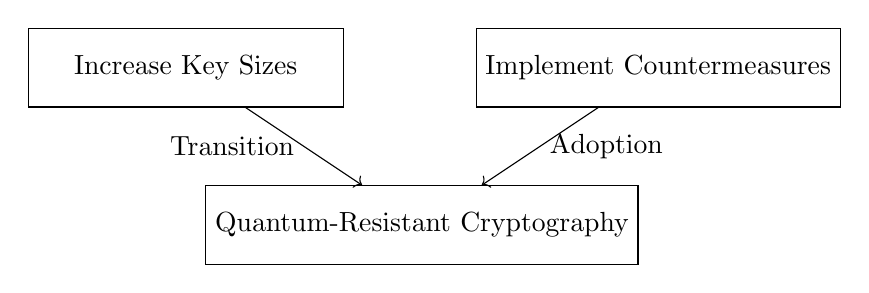
\begin{tikzpicture}
        % Nodes
        \node[draw, rectangle, minimum width=4cm, minimum height=1cm] (keysize) at (0, 0) {Increase Key Sizes};
        \node[draw, rectangle, minimum width=4cm, minimum height=1cm] (countermeasures) at (6, 0) {Implement Countermeasures};
        \node[draw, rectangle, minimum width=4cm, minimum height=1cm] (quantum) at (3, -2) {Quantum-Resistant Cryptography};
        
        % Arrows
        \draw[->] (keysize) -- (quantum) node[midway, left] {Transition};
        \draw[->] (countermeasures) -- (quantum) node[midway, right] {Adoption};
    \end{tikzpicture}
    \caption{Diagram illustrating mitigation strategies for RSA vulnerabilities.}\label{fig:mitigation_strategies}
\end{figure}


\chapter{Quantum Mechanics: The Foundation of Quantum Computing}
Quantum mechanics is the branch of physics that describes the behavior of matter and energy at the smallest scales, such as atoms and subatomic particles. It forms the theoretical foundation of quantum computing, enabling the development of algorithms that outperform classical counterparts for specific problems.

\section{Principles of Quantum Mechanics}
Quantum mechanics is governed by several key principles that distinguish it from classical physics:

\begin{itemize}
    \item \textbf{Superposition:} 
    Superposition is a fundamental principle of quantum mechanics that allows quantum systems to exist in multiple states simultaneously. In the context of quantum computing, a quantum bit (qubit) can represent both \( |0\rangle \) and \( |1\rangle \) at the same time, unlike classical bits that can only represent one state at a time. Mathematically, a qubit in superposition is represented as:
    \[
    |\psi\rangle = \alpha |0\rangle + \beta |1\rangle,
    \]
    where \( \alpha \) and \( \beta \) are complex numbers satisfying \( |\alpha|^2 + |\beta|^2 = 1 \). This property enables quantum computers to process a vast number of possibilities simultaneously, leading to exponential speedups for certain types of problems.
    \begin{figure}[H]
        \centering
            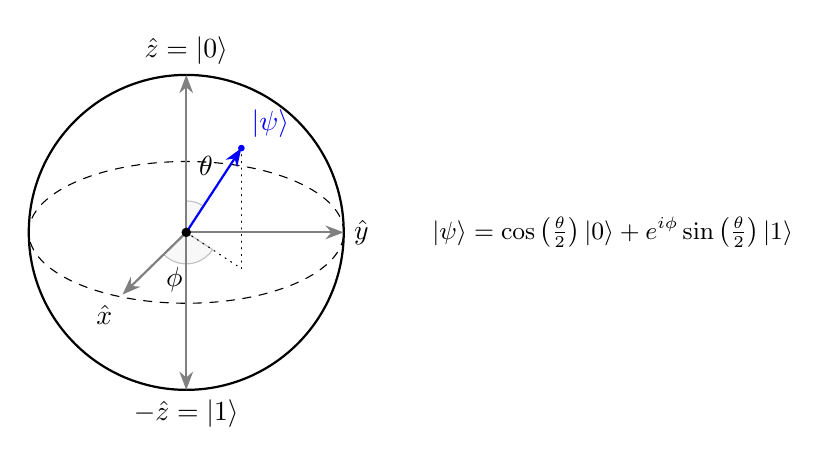
\begin{tikzpicture}[line cap=round, line join=round, >=Stealth]
            
            % Draw the outer sphere
            \draw[thick] (0,0) circle (2cm);
            
            % Draw the equatorial plane (dashed ellipse)
            \draw[dash pattern=on 3pt off 3pt] (0,0) ellipse (2cm and 0.9cm);
            
            % Highlight angles
            \draw[shift={(0,0)}, lightgray, fill, fill opacity=0.1] (0,0) -- (56.7:0.4) arc (56.7:90:0.4) -- cycle;
            \draw[shift={(0,0)}, lightgray, fill, fill opacity=0.1] (0,0) -- (-135.7:0.4) arc (-135.7:-33.2:0.4) -- cycle;
            
            % Axes
            \draw[->, thick, gray] (0,0) -- (0,2) node[anchor=south, black] {$\hat{z}=|0\rangle$};
            \draw[->, thick, gray] (0,0) -- (2,0) node[anchor=west, black] {$\hat{y}$};
            \draw[->, thick, gray] (0,0) -- (-0.81,-0.79) node[anchor=north east, black] {$\hat{x}$};
            \draw[->, thick, gray] (0,0) -- (0,-2) node[anchor=north, black] {$-\hat{z}=|1\rangle$};
            
            % Qubit state vector
            \draw[thick, ->, blue] (0,0) -- (0.7,1.07) node[anchor=south west] {$|\psi\rangle$};
            
            % Projection lines
            \draw[dotted] (0.7,1.07) -- (0.7,-0.46);
            \draw[dotted] (0,0) -- (0.7,-0.46);
            
            % Angle labels
            \node at (-0.15,-0.6) {$\phi$};
            \node at (0.25,0.85) {$\theta$}; % Adjusted theta position slightly to the right
            
            % State label moved to the side
            \node[align=left, font=\small, anchor=west] at (3,0) {$|\psi\rangle = \cos\left(\frac{\theta}{2}\right)|0\rangle + e^{i\phi}\sin\left(\frac{\theta}{2}\right)|1\rangle$};
            
            % Markers
            \draw[fill] (0,0) circle (1.5pt); % Origin
            \draw[fill, blue] (0.7,1.07) circle (1pt); % Qubit state
        \end{tikzpicture}
        \caption{Representation of a qubit on the Bloch sphere, showing the state \( |\psi\rangle = \cos\left(\frac{\theta}{2}\right)|0\rangle + e^{i\phi}\sin\left(\frac{\theta}{2}\right)|1\rangle \) with angles \( \theta \) and \( \phi \). The vector \( |\psi\rangle \) is shown in blue, illustrating that the atom is in a superposition of states \( |0\rangle \) and \( |1\rangle \) simultaneously.}
        \end{figure}

    \begin{figure}[H]
        \centering
        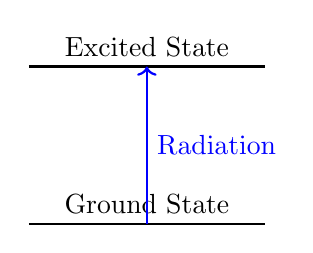
\begin{tikzpicture}
            % Energy levels
            \draw[thick] (0,0) -- (3,0) node[midway, above] {Ground State};
            \draw[thick] (0,2) -- (3,2) node[midway, above] {Excited State};
            % Electron transition
            \draw[->, thick, blue] (1.5,0) -- (1.5,2) node[midway, right] {Radiation};
        \end{tikzpicture}
        \caption{Electron transition from ground state to excited state upon exposure to radiation.}
    \end{figure}

    \item \textbf{Entanglement:} 
    Entanglement is a unique quantum phenomenon where two or more quantum particles become interconnected in such a way that the state of one particle is directly related to the state of the other, regardless of the distance between them. For example, the entangled state of two qubits can be represented as:
    \[
    |\psi\rangle = \frac{1}{\sqrt{2}} \left( |00\rangle + |11\rangle \right).
    \]
    This correlation persists even if the particles are separated by vast distances. In quantum computing, entanglement is used to create highly efficient communication and computation protocols.

    \begin{figure}[H]
        \centering
        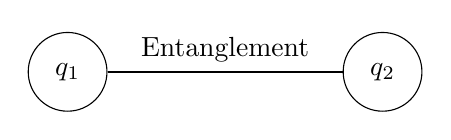
\begin{tikzpicture}
            % Nodes
            \node[circle, draw, minimum size=1cm] (q1) at (0,0) {\( q_1 \)};
            \node[circle, draw, minimum size=1cm] (q2) at (4,0) {\( q_2 \)};
            % Connection
            \draw[thick] (q1) -- (q2) node[midway, above] {Entanglement};
        \end{tikzpicture}
        \caption{Illustration of entangled qubits \( q_1 \) and \( q_2 \).}
    \end{figure}

    \item \textbf{Quantum Interference:} 
    Quantum interference arises from the wave-like nature of quantum particles. When quantum states overlap, their probability amplitudes can interfere constructively or destructively. Constructive interference amplifies the probability of correct solutions, while destructive interference cancels out incorrect ones. For example, in a quantum algorithm, the interference can be represented as:
    \[
    |\psi\rangle = \frac{1}{\sqrt{2}} \left( |0\rangle + |1\rangle \right) + \frac{1}{\sqrt{2}} \left( |0\rangle - |1\rangle \right) = |0\rangle.
    \]

    \begin{figure}[H]
        \centering
        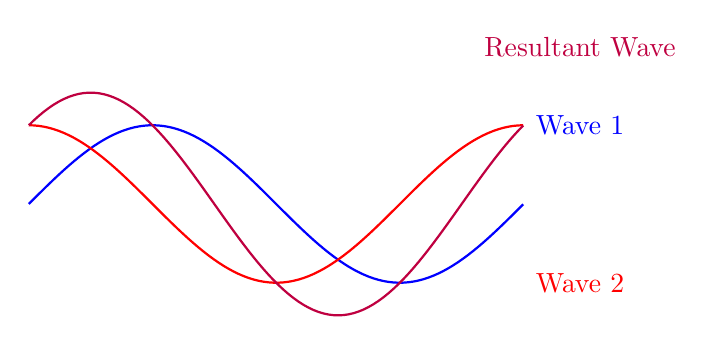
\begin{tikzpicture}
            % Waves
            \draw[thick, blue, domain=0:6.28, samples=100] plot (\x, {sin(\x r)});
            \draw[thick, red, domain=0:6.28, samples=100] plot (\x, {cos(\x r)});
            \draw[thick, purple, domain=0:6.28, samples=100] plot (\x, {sin(\x r) + cos(\x r)});
            % Labels
            \node[blue] at (7, 1) {Wave 1};
            \node[red] at (7, -1) {Wave 2};
            \node[purple] at (7, 2) {Resultant Wave};
        \end{tikzpicture}
        \caption{Constructive interference of quantum states.}
    \end{figure}

    \item \textbf{Measurement:} 
    Measurement in quantum mechanics is the process of observing a quantum system, which causes the system to collapse into a definite state. Before measurement, a quantum system exists in a superposition of all possible states, each with a certain probability amplitude. Upon measurement, the system randomly collapses into one of these states. For example, measuring the state:
    \[
    |\psi\rangle = \frac{1}{\sqrt{2}} |0\rangle + \frac{1}{\sqrt{2}} |1\rangle,
    \]
    will yield \( |0\rangle \) or \( |1\rangle \) with equal probability \( \frac{1}{2} \).

    \begin{figure}[H]
        \centering
        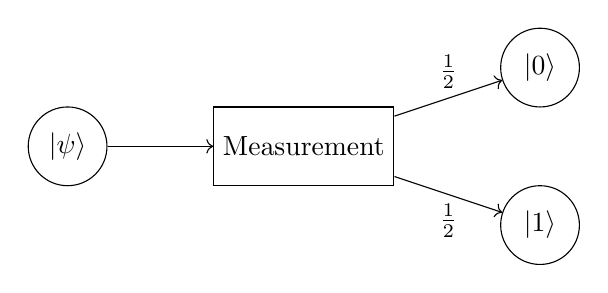
\begin{tikzpicture}
            % Qubit
            \node[circle, draw, minimum size=1cm] (qubit) at (0,0) {\( |\psi\rangle \)};
            % Measurement
            \node[rectangle, draw, minimum width=2cm, minimum height=1cm] (measure) at (3,0) {Measurement};
            % Outcomes
            \node[circle, draw, minimum size=1cm] (out1) at (6,1) {\( |0\rangle \)};
            \node[circle, draw, minimum size=1cm] (out2) at (6,-1) {\( |1\rangle \)};
            % Arrows
            \draw[->] (qubit) -- (measure);
            \draw[->] (measure) -- (out1) node[midway, above] {\( \frac{1}{2} \)};
            \draw[->] (measure) -- (out2) node[midway, below] {\( \frac{1}{2} \)};
        \end{tikzpicture}
        \caption{Measurement collapsing a qubit into a definite state.}
    \end{figure}
\end{itemize}

\section{Mathematical Framework of Quantum Mechanics}
The mathematical framework of quantum mechanics is based on linear algebra and complex vector spaces. The key notations and concepts include:
\begin{itemize}

    \item \textbf{Schrödinger Equation:} The time evolution of a quantum system is governed by the Schrödinger equation:
    \[
    i\hbar \frac{\partial}{\partial t} |\psi(t)\rangle = \hat{H} |\psi(t)\rangle,
    \]
    where \( \hat{H} \) is the Hamiltonian operator representing the total energy of the system.

    \item \textbf{Probability Amplitudes:} The probability of measuring a particular outcome is given by the square of the amplitude of the corresponding state vector component. For example, the probability of measuring \( |0\rangle \) in the state \( |\psi\rangle = \alpha |0\rangle + \beta |1\rangle \) is \( |\alpha|^2 \).
    
    \item \textbf{State Vectors:} The state of a quantum system is represented by a vector in a complex Hilbert space, denoted as \( |\psi\rangle \). For example, a single qubit state can be written as:
    \[
    |\psi\rangle = \alpha |0\rangle + \beta |1\rangle,
    \]
    where \( \alpha, \beta \in \mathbb{C} \) and \( |\alpha|^2 + |\beta|^2 = 1 \).

    \item \textbf{Bra-Ket Notation:} Quantum states are expressed using Dirac's bra-ket notation:
    \begin{itemize}
        \item \( |\psi\rangle \): A column vector (ket) representing the state.
        \item \( \langle\psi| \): A row vector (bra), the Hermitian conjugate of \( |\psi\rangle \).
    \end{itemize}
    The inner product of two states \( |\psi\rangle \) and \( |\phi\rangle \) is written as \( \langle\psi|\phi\rangle \), and the outer product is \( |\psi\rangle\langle\phi| \).

    \item \textbf{Operators:} Physical observables, such as position and momentum, are represented by Hermitian operators acting on state vectors. For example, the Pauli-X operator is:
    \[
    X = \begin{bmatrix}
    0 & 1 \\
    1 & 0
    \end{bmatrix}.
    \]

    \item \textbf{Tensor Products:} Multi-qubit systems are represented using tensor products. For example, the state of two qubits \( |\psi_1\rangle \) and \( |\psi_2\rangle \) is:
    \[
    |\psi\rangle = |\psi_1\rangle \otimes |\psi_2\rangle.
    \]

    \item \textbf{Unitary Operators:} Quantum gates are represented by unitary matrices \( U \), satisfying \( U^\dagger U = I \), where \( U^\dagger \) is the conjugate transpose of \( U \) and \( I \) is the identity matrix.
\end{itemize}

\section{Quantum Gates and Circuits}
Quantum gates are the building blocks of quantum circuits, analogous to classical logic gates. They manipulate qubits and perform operations based on the principles of quantum mechanics:

\subsection{Single-Qubit Gates}
Single-qubit gates operate on a single qubit and are represented by \( 2 \times 2 \) unitary matrices. Examples include:
\begin{itemize}
    \item \textbf{Pauli-X Gate:} Acts as a quantum NOT gate, flipping the state of a qubit. Its matrix representation is:
    \[
    X = \begin{bmatrix}
    0 & 1 \\
    1 & 0
    \end{bmatrix}.
    \]
    \item \textbf{Hadamard Gate:} Creates a superposition of states. Its matrix representation is:
    \[
    H = \frac{1}{\sqrt{2}} \begin{bmatrix}
    1 & 1 \\
    1 & -1
    \end{bmatrix}.
    \]
    \item \textbf{Phase Gate:} Introduces a phase shift. For example, the \( S \)-gate is:
    \[
    S = \begin{bmatrix}
    1 & 0 \\
    0 & i
    \end{bmatrix}.
    \]
\end{itemize}

\subsection{Multi-Qubit Gates}
Multi-qubit gates operate on multiple qubits and are essential for creating entanglement and performing complex quantum operations:
\begin{itemize}
    \item \textbf{CNOT Gate:} A controlled-NOT gate flips the target qubit if the control qubit is \( |1\rangle \). Its matrix representation is:
    \[
    \text{CNOT} = \begin{bmatrix}
    1 & 0 & 0 & 0 \\
    0 & 1 & 0 & 0 \\
    0 & 0 & 0 & 1 \\
    0 & 0 & 1 & 0
    \end{bmatrix}.
    \]
    \item \textbf{Toffoli Gate:} A controlled-controlled-NOT gate, which flips the target qubit if both control qubits are \( |1\rangle \).
\end{itemize}

\subsection{Quantum Circuits}
A quantum circuit is a sequence of quantum gates applied to qubits to perform a computation. Mathematically, the overall operation of a quantum circuit is represented by the product of the unitary matrices of its gates. The output is obtained by measuring the qubits, collapsing their states into classical bits.

\section{Relevance to Quantum Computing}
Quantum mechanics provides the theoretical underpinnings for quantum computing, enabling the development of powerful algorithms. For example:
\begin{itemize}
    \item \textbf{Shor's Algorithm:} Efficiently factors integers by leveraging quantum Fourier transforms.
    \item \textbf{Grover's Algorithm:} Provides a quadratic speedup for unstructured search problems.
\end{itemize}
By leveraging principles such as superposition, entanglement, and interference, quantum computers can solve problems that are intractable for classical computers.

\section{Challenges in Quantum Mechanics for Computing}
Despite its potential, quantum mechanics introduces challenges for quantum computing:
\begin{itemize}
    \item \textbf{Decoherence:} Quantum states are fragile and can lose coherence due to interactions with the environment, leading to errors in computation.
    \item \textbf{Error Correction:} Quantum error correction codes, such as the surface code, are required to mitigate the effects of noise and decoherence. These codes rely on encoding logical qubits into multiple physical qubits.
    \item \textbf{Scalability:} Building large-scale quantum computers with many qubits while maintaining coherence and low error rates is a complex engineering problem.
\end{itemize}

This chapter establishes the connection between quantum mechanics and quantum computing, highlighting the transformative potential of this interdisciplinary field and the challenges that must be overcome to realize its full potential.

\chapter{Existing Methods for Breaking RSA Before Quantum Computing}
Before the advent of quantum computing, several classical methods were explored to break RSA encryption. These methods, while not as efficient as quantum algorithms, posed potential threats under certain conditions. This chapter discusses the existing systems and techniques used to attack RSA encryption prior to the emergence of quantum computing.

\section{Brute Force Attacks}
Brute force attacks involve systematically trying all possible private keys to decrypt a message. However, due to the large key sizes used in RSA (typically 2048 bits or more), brute force attacks are computationally infeasible with classical computers.

\section{Mathematical Factorization Algorithms}
The security of RSA relies on the difficulty of factoring large integers. Several classical algorithms have been developed to factorize numbers, including:
\begin{itemize}
    \item \textbf{Trial Division:} A basic method that tests divisibility by smaller numbers, but it is highly inefficient for large integers.
    \item \textbf{Pollard's Rho Algorithm:} A probabilistic algorithm that works well for smaller numbers but struggles with large RSA keys.
    \item \textbf{Quadratic Sieve:} One of the fastest classical algorithms for factoring integers up to 100 digits.
    \item \textbf{General Number Field Sieve (GNFS):} The most efficient classical algorithm for factoring large integers, used in practical attacks on RSA with smaller key sizes.
\end{itemize}

\section{Side-Channel Attacks}
Side-channel attacks exploit physical implementations of RSA rather than its mathematical foundation. Examples include:
\begin{itemize}
    \item \textbf{Timing Attacks:} Measuring the time taken for cryptographic operations to infer private keys.
    \item \textbf{Power Analysis:} Observing power consumption patterns during encryption or decryption.
    \item \textbf{Electromagnetic Analysis:} Capturing electromagnetic emissions to extract sensitive information.
\end{itemize}

\section{Distributed Computing Efforts}
Projects like the RSA Factoring Challenge encouraged distributed computing efforts to factorize RSA keys. While these efforts demonstrated the vulnerability of smaller key sizes, they were not practical for breaking modern RSA implementations with sufficiently large keys.

\section{Limitations of Classical Methods}
Despite these methods, breaking RSA encryption with classical computers remains infeasible for adequately large key sizes. The computational resources and time required grow exponentially with key size, ensuring the security of RSA against classical attacks.

While RSA encryption has been a reliable cryptographic standard, it is not without limitations. The primary challenge lies in its reliance on the difficulty of integer factorization. With the advent of quantum computing, this foundational assumption is under threat, as quantum algorithms like Shor's algorithm can efficiently solve the integer factorization problem.

\chapter{Drawbacks of Existing Methods}
While existing methods for breaking RSA encryption have been extensively studied, they come with significant drawbacks that limit their practicality and effectiveness. This chapter discusses the key limitations of these methods:

\section{Brute Force Attacks}
\begin{itemize}
    \item \textbf{Exponential Time Complexity:} The time required to test all possible keys grows exponentially with key size, making brute force attacks infeasible for modern RSA implementations.
    \item \textbf{Resource Intensive:} Brute force attacks require substantial computational resources, which are often unavailable or impractical to deploy.
\end{itemize}

\section{Mathematical Factorization Algorithms}
\begin{itemize}
    \item \textbf{Inefficiency for Large Keys:} Classical factorization algorithms, such as the General Number Field Sieve (GNFS), become increasingly inefficient as the size of the RSA key increases.
    \item \textbf{High Computational Cost:} These algorithms demand significant computational power and time, limiting their applicability to smaller key sizes.
\end{itemize}

\section{Side-Channel Attacks}
\begin{itemize}
    \item \textbf{Dependency on Physical Access:} Side-channel attacks often require physical access to the cryptographic device, which is not always feasible.
    \item \textbf{Mitigation Techniques:} Modern cryptographic implementations include countermeasures to reduce the effectiveness of side-channel attacks, such as constant-time algorithms and noise injection.
\end{itemize}

\section{Distributed Computing Efforts}
\begin{itemize}
    \item \textbf{Scalability Issues:} Distributed computing efforts face challenges in scaling to factorize larger RSA keys due to the exponential growth in computational requirements.
    \item \textbf{Coordination Overhead:} Managing and coordinating large-scale distributed systems introduces additional complexity and overhead.
\end{itemize}

\section{General Limitations}
\begin{itemize}
    \item \textbf{Reliance on Classical Computing:} All existing methods are constrained by the limitations of classical computing, which cannot efficiently solve the integer factorization problem for large key sizes.
    \item \textbf{Inability to Address Quantum Threats:} These methods do not account for the advancements in quantum computing, which pose a more significant threat to RSA encryption.
\end{itemize}

These drawbacks highlight the need for more advanced approaches, such as quantum-resistant cryptographic systems, to address the vulnerabilities of RSA encryption in the face of evolving computational capabilities.

\chapter{Quantum Computing: A Paradigm Shift}
Quantum computing represents a revolutionary shift in computational capabilities, leveraging principles of quantum mechanics such as superposition and entanglement. This chapter explores the basics of quantum computing and highlights how it differs from classical computing, particularly in solving problems like integer factorization.

\chapter{Shor's Algorithm and Its Impact on RSA}
Shor's algorithm is a quantum algorithm that can factorize large integers exponentially faster than classical algorithms. This chapter delves into the workings of Shor's algorithm and explains how it directly undermines the security of RSA encryption, making it vulnerable to quantum attacks.

\chapter{Implications of Quantum Computing on Cryptography}
The ability of quantum computers to break RSA encryption has far-reaching implications for cryptography. This chapter discusses the potential risks to digital security, including compromised financial transactions, data breaches, and threats to national security, emphasizing the urgency of addressing these challenges.

\chapter{Advantages of Proposed System}
The proposed quantum-resistant cryptographic systems offer several advantages:
\begin{itemize}
    \item Enhanced security against quantum attacks, ensuring the confidentiality of sensitive information.
    \item Compatibility with existing communication protocols, allowing for a smoother transition to quantum-resistant systems.
    \item Scalability for future cryptographic needs, addressing the growing demand for secure communication in the quantum era.
    \item Reduced risk of data breaches and financial fraud caused by quantum-enabled attacks.
\end{itemize}

\chapter{Application}
Quantum-resistant cryptographic systems have a wide range of applications, including:
\begin{itemize}
    \item Securing financial transactions and online banking systems.
    \item Protecting sensitive government and military communications.
    \item Ensuring the privacy of personal data in healthcare and other industries.
    \item Safeguarding intellectual property and trade secrets in the corporate sector.
    \item Enabling secure communication in emerging technologies such as the Internet of Things (IoT) and autonomous vehicles.
\end{itemize}

\chapter{Future Enhancement}
The advent of quantum computing poses a significant challenge to traditional cryptographic systems like RSA encryption. However, it also drives innovation in the field of cryptography, leading to the development of quantum-resistant algorithms. Future enhancements in this area include:
\begin{itemize}
    \item Standardizing quantum-resistant algorithms to ensure global adoption and interoperability.
    \item Improving the efficiency and performance of quantum-resistant cryptographic systems to meet real-world demands.
    \item Conducting extensive research to identify and mitigate potential vulnerabilities in proposed systems.
\end{itemize}

\chapter{Conclusion}
In conclusion, the transition to quantum-resistant cryptography is essential to mitigate the risks posed by quantum computing. By adopting these advanced systems, we can ensure the continued security of sensitive information and maintain trust in digital communication in the quantum era.

% \chapter*{References}
% \begin{enumerate}
%     \item Shor, P. W. (1994). Algorithms for quantum computation: Discrete logarithms and factoring. \textit{Proceedings 35th Annual Symposium on Foundations of Computer Science}.
%     \item Rivest, R. L., Shamir, A., \& Adleman, L. (1978). A method for obtaining digital signatures and public-key cryptosystems. \textit{Communications of the ACM}.
%     \item National Institute of Standards and Technology (NIST). Post-Quantum Cryptography. \url{https://csrc.nist.gov/Projects/Post-Quantum-Cryptography}.
% \end{enumerate}

\begin{thebibliography}{9}
    \bibitem{Rivest1978}
    Rivest, R., Shamir, A., \& Adleman, L. (1978). 
    \textit{A Method for Obtaining Digital Signatures and Public-Key Cryptosystems}. 
    Communications of the ACM, 21(2), 120--126. 
    CiteSeerX 10.1.1.607.2677.\space doi:\href{https://doi.org/10.1145/359340.359342}{10.1145/359340.359342}. S2CID 2873616. 
    Archived from the original (PDF) on 2023--01--27.\@ 
    Available at: \url{http://people.csail.mit.edu/rivest/Rsapaper.pdf}.
\end{thebibliography}

\end{document}